\documentclass[12pt]{article}
\usepackage[utf8]{inputenc}
\usepackage[T5]{fontenc}
\usepackage{graphicx,a4wide,framed,amssymb}
\usepackage{tikz}
\usetikzlibrary{decorations,decorations.pathmorphing,shadows}

\newcommand{\source}[1]{\begin{flushright}\emph{[#1]}\end{flushright}}

\newcommand{\MakeScribeTop}[1]{
\noindent
\begin{framed}
\noindent
 Algorithmique Avancée 2018
 \hfill
 École Centrale-Supélec
 \\[1em]
 \centerline{ \Large
#1
 }
 \\[1em]
\centerline{  \it Christoph Dürr, Nguyễn Kim Thắng}
\end{framed}
}



\begin{document}
    \MakeScribeTop{PC3 : Programmation dynamique 2}

    \section{Trianguler un polygone convexe}

    On vous donne un polygone convexe formé des points $p_0,\ldots,p_{n-1}$ dans l'ordre normal, et tel que pour tout $i$, le point $p_{i+1}$ ne soit pas sur la droite définie par $p_i$ et $p_{i+2}$ (les indices sont pris modulo $n$).
    Le but est de relier les points avec des segments de longueur totale minimale, pour décomposer le polygone en triangles.
    Donnez un programme dynamique pour ce problème.

\begin{figure}[ht]
\begin{center}
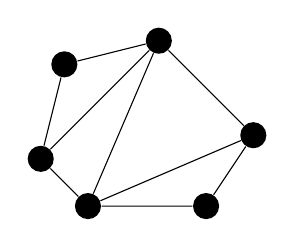
\begin{tikzpicture}[scale=0.3]
\node[circle,fill=black] (a) at (5,7)  {};
\node[circle,fill=black] (b) at (1,6)  {};
\node[circle,fill=black] (c) at (0,2)  {};
\node[circle,fill=black] (d) at (2,0)  {};
\node[circle,fill=black] (e) at (7,0)  {};
\node[circle,fill=black] (f) at (9,3)  {};
\draw (f) -- (a) -- (b) -- (c) -- (d) -- (e) -- (f) -- (d) -- (a) -- (c);
\end{tikzpicture}
\end{center}
\caption{Un polygone et sa triangulation (pas forcément optimale).}
\end{figure}

\section{Plus grand carré dans une grille}

Étant donnée une grille de dimension $n\times m$ aux cases colorés en blanc ou noir, trouvez un plus grand carré dans la grille (intersection de lignes $[i,i+k]$ et colonnes $[j,j+k]$ pour des entiers $i,j,k$) qui soit entièrement blanc.


\section{Ensemble indépendant de poids maximum dans un arbre}

Un ensemble $S\subseteq V$ est indépendant dans le graphe $G(V,E)$ si les sommets de $S$ ne sont pas reliés par une arête.
Étant donné une pondération $w:V\rightarrow \mathbb N$, trouvez un ensemble indépendant $S$ qui maximise $\sum_v\in S w_v$.  C'est un problème NP-difficile, mais très facile pour les arbres.  Donnez un programme dynamique de complexité linéaire pour ce problème.  Indice: choisissez un sommet arbitraire comme racine pour définir la notion de sous-arbre.

\section{Plus long chemin dans un arbre}

Étant donné un arbre $G(V,E)$ calculez la longueur du plus long chemin dans l'arbre.  Ceci peut être fait par deux parcours successifs en profondeur, mais pour cet exercice donnez un programme dynamique.

\section{Jeux avec des pièces alignées}

Vous jouez un jeu avec votre nièce Sigrid.  Sur la table sont alignées des pièces valant chacune une différente sommet d'argent, disons $w_1$ à $w_n$ en prenant les pièces de gauche à droite.  À tour de rôle, chacun de vous prend une des deux pièces extrêmes, toute à gauche ou toute à droite.  Sigrid commence. Quand il n'y a plus de pièces sur la table, vous comparez le total des pièces ramassées.  La personne avec la plus grande somme gagne.
\begin{figure}[ht]
\begin{center}
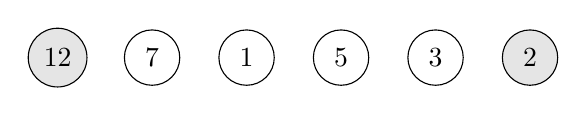
\begin{tikzpicture}[scale=0.3]
\node[circle,draw,minimum size=2em,fill=gray!20] at (0,0)  {12};
\node[circle,draw,minimum size=2em] at (4,0)  {7};
\node[circle,draw,minimum size=2em] at (8,0)  {1};
\node[circle,draw,minimum size=2em] at (12,0)  {5};
\node[circle,draw,minimum size=2em] at (16,0)  {3};
\node[circle,draw,minimum size=2em,fill=gray!20] at (20,0)  {2};
\end{tikzpicture}
\end{center}
\caption{Une configuration du jeux. Le prochaine joueur peut prendre une des deux pièces grises.}
\end{figure}


\section{Ski alpin}

Considérons une piste de ski alpin, modélisé par le plan euclidien, où la gravitation agit dans la direction $-y$. Vous débutez votre descente en le  point $(x_0,y_0)$. Le long de la piste se trouvent des paires de drapeaux, la $i$-ième paire est composé des drapeaux en $(x_i,y_i)$ et $(x'_i,y_i)$, avec $x_i < x'_i$ et $y_0 > y_1 > \ldots y_n > 0$.  Votre but est de descendre le plus rapidement possible.  Pour cela déterminez un plus court chemin du point de départ à la ligne d'arrivée $\{(x,0):x\in \mathbb R\}$ en passant entre les drapeaux de chaque paire.  Ce plus court chemin sera linéaire par morceaux et donc on ne tient pas compte des virages à effectuer en arrondi.

Donnez un programme dynamique pour ce problème.

\end{document}